\documentclass[10pt]{article}

%AMS-TeX packages
\usepackage{amssymb,amsmath,amsthm} 
%geometry (sets margin) and other useful packages
\usepackage[margin=1.25in]{geometry}
\usepackage{graphicx,ctable,booktabs}
\usepackage{verbatim}
\usepackage{color}
\usepackage{listings}
\lstset{ %
language=C,                % choose the language of the code
basicstyle=\footnotesize,       % the size of the fonts that are used for the code
numbers=left,                   % where to put the line-numbers
numberstyle=\footnotesize,      % the size of the fonts that are used for the line-numbers
stepnumber=1,                   % the step between two line-numbers. If it is 1 each line will be numbered
numbersep=5pt,                  % how far the line-numbers are from the code
backgroundcolor=\color{white},  % choose the background color. You must add \usepackage{color}
showspaces=false,               % show spaces adding particular underscores
showstringspaces=false,         % underline spaces within strings
showtabs=false,                 % show tabs within strings adding particular underscores
frame=single,           % adds a frame around the code
tabsize=2,          % sets default tabsize to 2 spaces
captionpos=b,           % sets the caption-position to bottom
breaklines=true,        % sets automatic line breaking
breakatwhitespace=false,    % sets if automatic breaks should only happen at whitespace
escapeinside={\%*}{*)}          % if you want to add a comment within your code
}

%
%Fancy-header package to modify header/page numbering 
%
\usepackage{fancyhdr}
\pagestyle{fancy}
%\addtolength{\headwidth}{\marginparsep} %these change header-rule width
%\addtolength{\headwidth}{\marginparwidth}
\lhead{CS 261 Project Report}
\chead{} 
\rhead{\thepage} 
\lfoot{\small Andrew Johnson and Scott Moore} 
\cfoot{} 
\rfoot{\footnotesize CS 261 Project Report} 
\renewcommand{\headrulewidth}{.3pt} 
\renewcommand{\footrulewidth}{.3pt}
\setlength\voffset{-0.25in}
\setlength\textheight{648pt}

\usepackage[square,numbers]{natbib}

%%%%%%%%%%%%%%%%%%%%%%%%%%%%%%%%%%%%%%%%%%%%%%%

\usepackage{trfrac}

\newcommand{\ruletext}[1]{{\scriptsize\textsf{#1}}}
\newcommand{\signrule}{\ruletext{SIGN}}
\newcommand{\confrule}{\ruletext{CONF}}
\newcommand{\assumprule}{\ruletext{ASSUMP}}
\newcommand{\tautorule}{\ruletext{TAUTO}}
\newcommand{\weakenrule}{\ruletext{WEAKEN}}
\newcommand{\implrule}{\ruletext{IMPL}}
\newcommand{\saysrule}{\ruletext{SAYS}}
\newcommand{\specrule}{\ruletext{SPEC}}
\newcommand{\sayssignrule}{\ruletext{SAYS SIGN}}
\newcommand{\saysconfrule}{\ruletext{SAYS CONF}}

\newcommand{\sign}[2]{\ensuremath{#1\;\textsf{signed}\;#2}}
\newcommand{\imp}[2]{\ensuremath{#1 \rightarrow #2}}
\newcommand{\says}[2]{\ensuremath{#1\;\textsf{says}\;#2}}
\newcommand{\confirms}[2]{\ensuremath{#1\;\textsf{confirms}\;#2}}
\newcommand{\ctxt}[0]{\ensuremath{\Gamma}}
\newcommand{\nil}[0]{\ensuremath{\cdot}}
\newcommand{\bnfsep}[0]{\ensuremath{\;\mid\;}}
\newcommand{\entails}[2]{\ensuremath{#1 \vdash #2}}
\newcommand{\pred}[2]{\ensuremath{\textsc{#1}(#2)}}
\newcommand{\subst}[2]{\ensuremath{[#1/#2]}}
\newcommand{\abs}[1]{\ensuremath{\forall x:\;#1}}
\newcommand{\rtcheck}[0]{\ensuremath{\textsf{Runtime check}}}
\newcommand{\with}[1]{\ensuremath{\;(\text{with } #1)}}
\newcommand{\todo}[1]{{\color{red}todo: {#1}}}

\begin{document}

\title{Authorization Logic in JOS}
\author{Andrew Johnson and Scott Moore}

\maketitle

\thispagestyle{empty}

\setlength\parindent{0em}
\setlength\parskip{1em}

\section{Introduction}
Access control in JOS is overly restrictive and mandatory. System calls that modify an environment may only be invoked by the the environment itself or its immediate ancestor. As a result, applications that do not have a clear hierarchical structure must use IPC for all inter-process communication. In particular, sharing memory requires per-page synchronization through IPC calls.

Authorization logics are a principled technique for implementing rule-based access control mechanisms.
They have several advantages over traditional OS access control mechanisms such as access control lists.
In particular, they allow principals to express access control decisions for which they do not have complete information.
Authorization logics also provide \emph{proof-carrying authorization}. That is, the capability to access a resource carries with it the set of authorization decisions that granted it.

We showed the feasibility of using authorization logic as an OS-level access control mechanism by implementing it in JOS. We found that its performance was comparable to existing mechanisms in JOS, particularly if the results of proof-checking are cached by the kernel.

\subsection{Related work}
Existing work on authorization logics has focused primarily on distributed systems.
More recently, \citet{Nexus} developed the Nexus operating system, which uses authorization logic to combine different trust bases for secure systems into a cohesive authorization system.
By aggressively caching evaluated proofs and avoiding cryptography by storing assertions in the kernel, Nexus achieves a 6\% overhead on a toy multi-tier webserver implementing a simple social networking site.
Nexus also describes a mechanism for enforcing state-based authorization policies in an authorization logic system.
Nexus supports \emph{authorities}, which verify authorization statements only when asked. Since the results of these checks cannot be reused, this mechanism can be used to support revocation and other dynamic authorization policies.
We incorporate a similar mechanism into our system.

Our authorization logic is based on \citet{Bauer}'s authorization logic extended with a primitive for dynamic authorization checks and cut elimination, which reduces the size of proofs.
More sophisticated authorization logics are given by \citet{AURA} and \citet{Garg}.

\section{Overview}

We replaced the current authorization mechanism for JOS system calls (\textsf{envid2env}) with a new mechanism based on authorization logic. Principals (environments) use a system call to specify an authorization goal which is used to mediate access to system calls affecting the environment.
An authorization goal is a formula in our authorization logic. Access is granted to any principal presenting a proof of the authorization goal. This is accomplished by a system call that registers a proof to be used for subsequent system calls. We describe the details of our JOS implementation in Section~\ref{sec:impl}.
If an environment does not specify an authorization goal, JOS's original parent-child authorization scheme is used.

Formulas in our logic have the following syntax: \\[1em]
\begin{tabular}{llcl}
\emph{principals} & R & ::= & $x$ \bnfsep $v$ \\
\emph{predicates} & P & ::= & $pred(R)$ \\
\emph{formulas} & F & ::= & $P$ \bnfsep \imp{F_1}{F_2} \bnfsep \abs{F} \bnfsep \sign{A}{F} \bnfsep \says{A}{F} \bnfsep \confirms{A}{F}\\
\emph{contexts} & \ctxt & ::= & \nil \bnfsep \ctxt,$F$ \\
\end{tabular} \\[1em]

Formulas include first order predicates over principals, implication, and universal quanitification over principals. Conjunction can be encoded as implication ($A \wedge B \rightarrow C \equiv A \rightarrow B \rightarrow C$). The remaining formulas describe a principal's beliefs. The formula \says{A}{F} can be interpreted as ``principal $A$ believes the formula $F$ to be true.'' In general, we can infer statements of this form by logical inference from the set of initial beliefs of the principal and the beliefs of other principals. We distinguish between two types of belief: these initial, or \emph{asserted}, beliefs and derived beliefs. \textsf{says} denotes derived beliefs, while \textsf{signed} and \textsf{confirms} represent asserted beliefs.

\textsf{signed} beliefs are irrevocable. In our system, environments assert irrevocable beliefs by registering them with the kernel via a system call.
\confirms{A}{F} is a new formula we are adding to the logic and corresponds with the authority abstraction in the Nexus system \cite{Nexus}. 
\confirms{A}{F} represents a run time authorization decision. \confirms{A}{F} is validated by invoking a decision procedure in $A$ that takes the authorization formula $F$ as input and returns true if $A$ believes $F$.
Crucially, checking the validity $\confirms{A}{F}$ does not create a reusable proof object.
This allows time-sensitive or revocable authorization decisions to be implemented on top of our simple logic without explicitly incorporating time or revocation as primitives.

\begin{figure}
\center
$\trfrac[\;\signrule]{\rtcheck}{\entails{\ctxt}{\sign{A}{F}}}$ \hfil
$\trfrac[\;\confrule]{\rtcheck}{\entails{\ctxt}{\confirms{A}{F}}}$ \hfil
$\trfrac[\;\assumprule]{F \in \ctxt}{\entails{\ctxt}{F}}$ \\[1em]

$\trfrac[\;\tautorule]{\entails{\ctxt}{F}}{\entails{\ctxt}{\says{A}{F}}}$ \hfil
$\trfrac[\;\weakenrule]{\entails{\ctxt,F_1}{F_2}}{\entails{\ctxt}{\imp{F_1}{F_2}}}$ \hfil
$\trfrac[\;\implrule]{\entails{\ctxt}{F_1} \quad \entails{\ctxt}{\imp{F_1}{F_2}}}{\entails{\ctxt}{F_2}}$ \\[1em]
$\trfrac[\;\sayssignrule]{\entails{\ctxt}{\sign{A}{F_1}} \quad \entails{\ctxt,F_1}{\says{A}{F_2}}}{\entails{\ctxt}{\says{A}{F_2}}}$ \hfil
$\trfrac[\;\saysconfrule]{\entails{\ctxt}{\confirms{A}{F_1}} \quad \entails{\ctxt,F_1}{\says{A}{F_2}}}{\entails{\ctxt}{\says{A}{F_2}}}$ \\[1em]
$\trfrac[\;\saysrule]{\entails{\ctxt}{\says{A}{F_1}} \quad \entails{\ctxt,F_1}{\says{A}{F_2}}}{\entails{\ctxt}{\says{A}{F_2}}}$ \hfil
$\trfrac[\;\specrule]{\entails{\ctxt}{\says{A}{(\abs{F_1})}} \quad \exists p:\;\entails{\ctxt,F_1\subst{p}{x}}{\says{A}{F_2}}}{\entails{\ctxt}{\says{A}{F_2}}}$
\caption{Inference rules of our authorization logic}
\label{fig:logic}
\end{figure}

The inference rules for our logic are given in Figure~\ref{fig:logic}. Rules \weakenrule{}, \implrule{}, \specrule{}, and \assumprule{} are standard.
The remaining rules are used to infer the beliefs of principals. \tautorule{} says that a principal will believe any objectively true statement. The \saysrule{} rule says that a principal believes anything that can be inferred by assuming its other beliefs are true. The \saysconfrule{} and \sayssignrule{} rules are similar, but refer to asserted beliefs, which are in turn validated by runtime checks.

\paragraph{Example} Suppose that principal $A$ wishes to delegate its authorization decisions to $B$. Then $A$ would assert \sign{A}{\imp{(\says{B}{\pred{OK}{Env}})}{\pred{OK}{Env}}}. Now for any principal $C$ authorized by $B$ (\says{B}{\pred{OK}{C}}), we can derive \says{A}{\pred{OK}{C}}.

\medskip
Our logic has two properties that make it (like NAL and \citet{Bauer}'s logic) particularly appropriate for use in an authorization system. First, because \saysrule{}, \saysconfrule{}, and \sayssignrule{} are specific to particular principals, the impact of a malicious or errant principal is limited to the authorization decisions that have been delegated to it.
Second, because our logic is constructive, proofs not only demonstrate the capability to access a resource, but an audit trail describing how that access was granted.

\section{Implementation}
\label{sec:impl}

We completed our implementation in three stages.  First, we formalized our logic in the Coq Proof Assistant.  Second, we ported the proof checker written in Coq to C as a stand-alone library.  Third, we integrated the library into the JOS operating system.

\subsection{Coq}
To help ensure the correctness of our proof checker, we first implemented it in the Coq Proof Assistant. This enabled us to prove that our proof checker was correct, as well as work out some of the implementation details in a strongly typed language.
For example, we initially used an environment to map variables in formulas to their instantiations. This made the proof checker overly complicated and replacing this environment with explicit substitution within formulas led to a far simpler implementation in both Coq and C.  Writing the proof checker in Coq allowed us to prove its soundness with respect to our formalized logic (in fact, using Coq's dependent types, our Coq proof checker returns a formal proof of the checked formula). We also used the Coq implementation to prototype the helper functions for constructing proofs that we used in our JOS implementation. The logic, proof checker, and examples were implemented in about 400 lines in Coq.

\subsection{C Library} \label{sec:clib}
To avoid the need to port runtime support for Coq to JOS, we translated our Coq proof checker to C by hand.
While this means that we do not have formal correctness guarantees, prototyping our implementation in Coq helped eliminate logical errors in our code. To guard against translation errors, we wrote a number of tests (now in \textsf{user/proof\_test.c}).  The C library implements the logic and inference rules given in Figure~\ref{fig:logic}.  For ease of use we also implemented constructors for primitive proofs, primitive formulas, principals, and for more complex, commonly used, proofs.  The Context, shown as $\Gamma$ in Figure \ref{fig:logic}, was implemented as a stack of formulas since the proof checker adds a formula to the context and, once it has been used, removes that formula.  Formulas and Proofs are represented as tagged \textsf{union}s of the primitive types together with an \textsf{enum} indicating the current type (another option would have been to use C++ classes).  

To simplify memory management, all constructors perform a deep copy of their input data structures. This means that a proof can be freed without worrying about the constituent subproofs and formulas.  To make this approach easy to implement, each of the data structures has a comparison function and a deep-copy function.  In addition, to ease debugging and introspection, each data structure can be printed (recursively) as a pre-formatted \LaTeX{ } string (which we used to generate the examples in this report).  In total, the library implementation consists of approximately 2600 lines of C, about half of which is test code.

\subsection{JOS Integration}\label{sec:jos}
The library described in section \ref{sec:clib} provides a logic and a method to create and check proofs defined in that logic.  In order to use this for authorization we needed to integrate it into an operating system.  We chose to use JOS for simplicity; the existing authorization mechanism was easy to replace.  We chose to focus on replacing environment to environment authentication.  In JOS, an environment is authorized to manipulate another only if it is the direct parent environment. We replace this with a more flexible model built on our authorization logic.  Essentially, to manipulate environment $A$, environment $B$ must provide a proof of a logical formula defined by $A$.  These proofs are checked by the JOS kernel. The modular design of our C library allowed us to more or less drop it into JOS as a library.  In order to facilitate this we essentially only needed to implement a JOS dynamic memory allocator (\textsf{malloc} and \textsf{free}) to replace the \textsf{stdlib} version.   In total we added about 350 lines of C to the kernel 200, of which was the proof checker.  In addition we added about 1650 lines in library functions and 1450 lines in user programs.

\subsubsection{New System Calls}\label{sec:joscalls}
\paragraph{$\textsf{sys\_set\_goal}$} Each environment can specify an authorization goal for itself using the system call $\textsf{sys\_set\_goal(Formula f)}$.
For example, environment $A$ can create a new formula $F = \pred{OK}{x}$ and bind it to its authorization goal by calling $\textsf{sys\_set\_goal}$.

\paragraph{$\textsf{sys\_set\_proof}$} To manipulate environment $A$ through a system call, environment $B$ must then provide a proof of $\says{A}{\pred{OK}{B}}$ ($F$ with $B$ substituted for $x$). $B$ specifies the proof to be used for authorization by invoking a second system call, $\textsf{sys\_set\_proof(Proof p)}$, before making the system call that would affect environment $A$.

When executing the system call, JOS checks whether $A$ has specified an authorization goal. If it has, the kernel checks that the proof given by $B$ is a valid proof of $A$'s authorization goal. Otherwise, the kernel uses JOS's original parent-child authorization mechanism.

\paragraph{$\textsf{sys\_sign\_formula}$} Environment $A$ can assert a static belief by calling $\textsf{sys\_sign\_formula(Formula f)}$. This adds $\sign{A}{f}$ to the kernel's context.
This context is used in lieu of digital signatures. When a proof references a signed formula, the kernel verifies it against this context to ensure its validity.

\paragraph{Example 1} Listing~\ref{code:attest} gives a simple example of these system calls in use. In it, environment $A$ binds $\pred{OK}{x}$ as its proof goal and asserts $OK(B)$. $B$ then constructors a proof (given in Figure~\ref{fig:attest}) that it is authorized to access $A$ and uses it to map a page into $A$.

\begin{figure}
\[
\trfrac[\;\sayssignrule]{\trfrac[\;\sayssignrule]{\rtcheck}{\sign{B}{\pred{OK}{A}}} \quad \trfrac[\;\tautorule]{\trfrac[\;\assumprule]{\rtcheck}{\pred{OK}{A}}}{\says{B}{\pred{OK}{A}}}}{\says{B}{\pred{OK}{A}}}
\]
\caption{Simple Attestation Proof}
\label{fig:attest}
\end{figure}

\begin{figure}
\lstset{language=C,caption={Environment $A$ constructs a proof goal, $F$, and signs $F(B)$.  Environment $B$ creates and uses a proof of $\says{A}{F(B)}$ depending on the fact that $A$ signed $F(B)$.},label=code:attest}
\begin{lstlisting}
// Constructed in A

// This is equivalent to [for all x, OK(x)]
// What will actually be proved is [A says OK(B)] where B has been substituted for x
Formula F = formula_pred(OK, x);
sys_set_goal(F);
sys_sign_formula(formula_subst(F, x, B));

// Constructed in B

// Proof of [A says F(B)]
Formula F_B_subst = formula_pred(OK, B);
Proof P  = says_from_signed(A, F_B_subst);
sys_set_proof(P);
...
// Map a page from B to A
sys_page_map(0, Bvaddr, A, Avaddr, perm);
\end{lstlisting}
\end{figure}

\paragraph{Example 2}
Suppose an environment wishes to accept as ``OK'' whatever another environment accepts as ``OK''.  This is a fairly common type of proof called delegation.  Consider the following example.  We have a parent environment, $P$, and two child environments, $C_1$ and $C_2$.
$C_2$ delegates to $P$.  $C_1$ uses this fact along with the fact that $\sign{P}{\pred{OK}{C_1}}$ to prove $\says{C_2}{\pred{OK}{C_1}}$.  This will allow $C_1$ to make system calls affecting $C_2$, such as $\textsf{sys\_page\_map}$.  A typical proof using delegation can be seen in Figure \ref{fig:delegation}.  We have added helper functions to create these proofs.  The use of these to construct a proof can be seen in Listing \ref{code:delegation}.

\begin{figure}
$C_2$ \textsf{delegates to} $P$:
\begin{center}
$\trfrac[\;\sayssignrule]{\trfrac[\;\signrule]{\rtcheck}{\sign{C_2}{\abs{\imp{\says{P}{\pred{OK}{v_{0}}}}{\pred{OK}{v_{0}}}}}} \quad \trfrac[\;\tautorule]{\trfrac[\;\assumprule]{\rtcheck}{\abs{\imp{\says{P}{\pred{OK}{v_{0}}}}{\pred{OK}{v_{0}}}}}}{\says{C_2}{\abs{\imp{\says{P}{\pred{OK}{v_{0}}}}{\pred{OK}{v_{0}}}}}}}{\says{C_2}{\abs{\imp{\says{P}{\pred{OK}{v_{0}}}}{\pred{OK}{v_{0}}}}}}$
\end{center}
$P$ \textsf{authorizes} $C_1$:
\begin{center} $\trfrac[\;\tautorule]{\trfrac[\;\implrule]{\trfrac[\;\sayssignrule]{\trfrac[\;\signrule]{\rtcheck}{\sign{P}{\pred{OK}{C_1}}} \quad \trfrac[\;\tautorule]{\trfrac[\;\assumprule]{\rtcheck}{\pred{OK}{C_1}}}{\says{P}{\pred{OK}{C_1}}}}{\says{P}{\pred{OK}{C_1}}} \quad \trfrac[\;\assumprule]{\rtcheck}{\imp{\says{P}{\pred{OK}{C_1}}}{\pred{OK}{C_1}}}}{\pred{OK}{C_1}}}{\says{C_2}{\pred{OK}{C_1}}}$
\end{center}
$\says{C_2}{\pred{OK}{C_1}}$:
\begin{center}
$\trfrac[\;\specrule]{C_2 \textsf{ delegates to } P \quad C_1 \quad P \textsf{ authorizes } C_1}{\says{C_2}{\pred{OK}{C_1}}}$
\end{center}
\caption{Delegation Proof}
\label{fig:delegation}
\end{figure}

\begin{figure}
\lstset{language=C,caption={Delegation using helper functions, proof sharing has been omitted},label=code:delegation}
\begin{lstlisting}
// Constructed in C2
Proof del = delegate_from_signed(C2, P, OK);  

// Constructed in parent
Formula pred = formula_pred(OK, C1);
Proof  perm = says_from_signed(P, pred);

// Constructed in C2
Proof  use_del = use_delegation(C2, P, C1, OK, del, perm);
\end{lstlisting}
\end{figure}

In Listing \ref{code:delegation}, $P_1$ is a proof that $C_2$ delegates to $P$ for the OK predicate, and is constructed in line 2 above.  $P_2$ begins with $\sign{P}{\pred{OK}{C_1}}$ and is then used together with $P_1$ to prove $\says{C_2}{\pred{OK}{C_1}}$.  There are runtime checks required by ``signed'' to verify the signatures, and by ``assump'' to verify that the given statement is in the context (note that this proof begins with an empty context, but that the proof checker adds to its context at runtime).  

\subsubsection{Runtime Verification}
During proof checking there are three runtime checks: context membership, signatures, and confirmations.  The first is straightforward list inclusion, and the second is implemented as a special case of the first.  The third, confirmation, relies on code that is defined by the confirming environment.  By making the system call, \textsf{sys\_set\_confirms\_upcall}, the confirming environment, $A$, can set a function that should be called to check any statement of the form $\confirms{A}{F}$.  At runtime a candidate Formula is passed into the upcall, which returns a boolean value.  In our implementation we run this code in the proof checker (in the kernel), assuming it is well behaved (terminates, does not abuse privilege).  A future implementation should restrict upcalls to well-behaved functions and check this property at runtime. Alternatively, an interuptable kernel could implement these upcalls through IPC. Nexus takes the latter approach.

\subsubsection{Proof Sharing}\label{sec:share}
It can be easier to construct a proof or parts of a proof in the environment which defines the goal to be proved.  In these cases the proofs need to be handed out to the provers.  To do this we created library functions to send and receive proofs.  These are implemented on top of IPC, adding handling of dynamically allocated data structures.  We can achieve the same result as in Listing \ref{code:attest} using proof sharing as seen in Listing \ref{code:share}.

\begin{figure}
\lstset{language=C,caption={Environment $A$ constructs a proof and sends it to environment $B$, which then uses the proof.},label=code:share}
\begin{lstlisting}
// Constructed in A
Formula F = formula_pred(OK, x);
sys_set_goal(F);
// This automatically calls sys_sign_formula when called from A
Proof P  = says_from_signed(A, formula_subst(F, x, B));
send_proof(B, P);

// Constructed in B
Proof P = receive_proof();
sys_set_proof(P);
...
// Map a page from B to A
sys_page_map(0, Bvaddr, A, Avaddr, perm);
\end{lstlisting}
\end{figure}

\subsubsection{Proof Caching}\label{sec:cache}
We implement a simple form of proof caching.  If the proof checker returns true, we add that proof's goal to a persistent context located in the kernel.  When a proof is checked we first check whether the proof's goal is already in the kernel's context.  If it is then we immediately return true.  Note that we should not cache any proofs using confirmation, since this is a dynamic runtime check.  In our prototype implementation of proof-caching we do not take this into account. The effects of caching can be seen in the Section~\ref{sec:eval}. Note that by default proof-caching is disabled (enable in \textsf{kern/env.c}, requires recompilation).

\subsubsection{User Programs}
We implemented several user space programs to test our authorization system. Here we give brief descriptions:
\setlength\parskip{0em}
\paragraph{prooftest} Contains tests for functions pertaining to building, printing, and copying Formulas and building, printing, copying, and checking Proofs.
\paragraph{prooftimertest} Implements infrastructure used for performance testing.
\paragraph{authtest} Builds and uses simple attestation proof as in Listing \ref{code:share}.
\paragraph{confirmstest} Sets a confirms up call and creates a proof that uses it.
\paragraph{fratricide} The parent environment forks 10 children.  Each one delegates to the parent.  The parent then spawns the 11th child, call him Killer, and signs a statement that Killer is OK.  The parent then exits gracefully, and Killer senselessly \textsf{sys\_env\_destroy}s the other 10 children before \textsf{sys\_env\_destroy}ing himself.
\paragraph{authmemmap} The parent environment forks 2 children.  Each delegates to the parent who then signs that the second environment is OK.  The second environment is then able to map a number of pages into the first environment with a single IPC message, which is used only for synchronization.  Previously each page would need to be shared via a separate IPC message.  (Note that occasionally this program runs into a race condition where the IPC message was received, but the receiving environment still page faults.  This appears to be unrelated to our authorization logic additions.)
\paragraph{authcompare} This program sets up the logic to compare mapping memory using runtime authorization and \textsf{sys\_page\_map} to using IPC.  The goal is to map 1000 pages from one environment to another.  The authorization logic setup is the same as in \textsf{authmemmap}.  When using IPC, the sender loops, calling \textsf{ipc\_send} and the receiver loops, calling \textsf{ipc\_receive}.
\setlength\parskip{1em}
\section{Evaluation}\label{sec:eval}
\subsection{Performance}
\begin{figure}
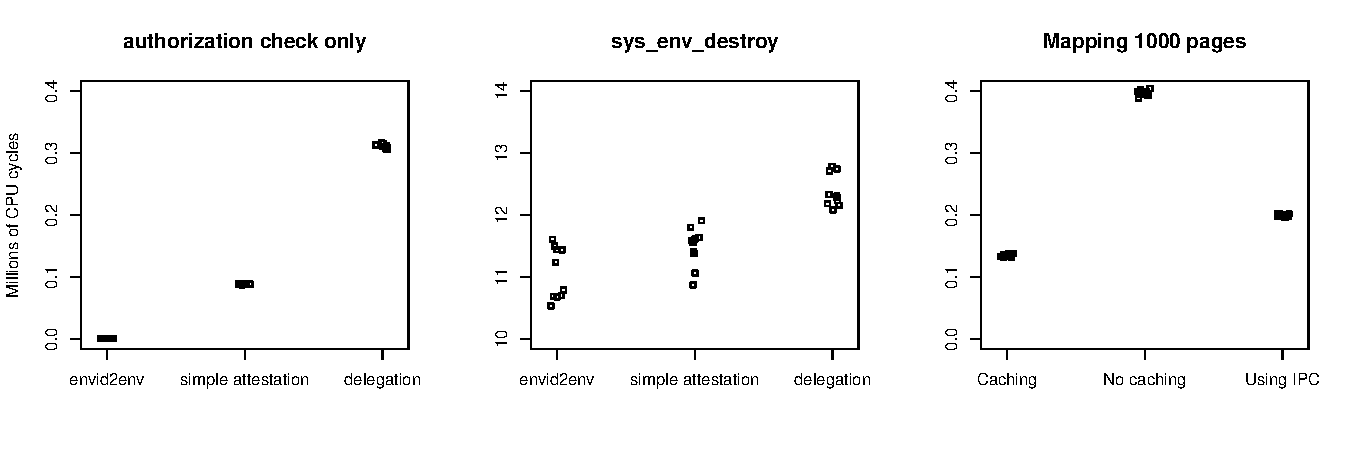
\includegraphics[width=\textwidth]{plots.pdf}
\caption{The left and center plots show the performance of authorization logic proof checking compared with previous JOS mechanism.  The right plot shows the effect of proof-caching and compares mapping 1,000 pages with our authorization checks to sending pages over IPC.}
\label{fig:perf}
\end{figure}
To evaluate the performance of the proof checker in the kernel we implemented a dummy system call that checks authorization and immediately returns. We also used this system call to debug proofs.  As seen in Figure~\ref{fig:perf}, we compared the performance of the existing parent/child check to checking the simple proof used in Listing~\ref{code:attest}, and against a more complex proof described in Figure~\ref{fig:delegation}.  We measured CPU cycles from within QEMU using $\textsf{rdtsc()}$. These were measured from the time the system call function was called in the kernel to the time it returns, and thus does not include any kernel crossings.  The left and center plots in Figure \ref{fig:perf} use no proof-caching, so this is roughly equivalent to checking a different proof in each system call.  The left plot in Figure \ref{fig:perf} shows the number of cycles for just the authentication checks.  Each circle is the average of 40,000 calls for \textsf{envid2env} and attestation and 1500 calls for delegation.  The center shows the number of cycles for the \textsf{sys\_env\_destroy} function call.  Each circle in this plot is a single call to \textsf{sys\_env\_destroy}. (Note that we made many other system calls prior to \textsf{sys\_env\_destroy} since the first system call took significantly longer in each case due to what we assume were cache effects).

The left plot in Figure \ref{fig:perf} shows a significant amount of slowdown.  The simple attestation is about 110 times slower than the simple parent/child check, and checking delegation is approximately 3.5 times slower than the simple check.  The proof for attestation can be seen in Figure~\ref{fig:attest} and the proof for delegation in Figure~\ref{fig:delegation}.  Each horizontal line is effectively either a runtime check or a run of the proof checker.  The simple proof has 4 checks while the delegation proof has 12, so, as expected, we see an approximately linear slowdown with increased proof complexity.  In the center of Figure~\ref{fig:perf} we see that the work done by a complex system call, such as \textsf{sys\_env\_destroy}, dominates the proof checking time with less than 5\% slow down for simple proof checking and less than 15\% slowdown for the delegation proof.  Note that the delegation proof is enabling environment interactions that would be impossible in the parent/child scheme, an environment can fall back on the fast parent/ child check by setting their goal to \textsf{NULL}.  Any scheme performing more complex checks would inevitably be slower, but we probably see additional slowdown as we trade performance for flexibility and generality. Furthermore, our current implementation performs a significant number of deep copies intended to simplify memory management. Optimizing away some of these copies could dramatically improve performance.

\subsubsection{Proof Caching}\label{sec:cacheperf}
Some of the performance losses in our system can be gained back without sacrificing functionality. A useful optimization in the Nexus operating system was proof-caching \cite{Nexus}.  For frequently used proofs we could cache the proof checker output in the kernel, or at least cache the parts that do not require dynamic runtime checks (everything but confirmation verifications). Another interesting possibility is for environments to provide proof-shortening services in user space. For example, an environment, $A$, when presented with a complex, valid complex proof of $\says{A}{F}$ could sign a copy of $F$, which can then be used in place of the original proof. We leave this as future work.

As discussed in Section~\ref{sec:cache} we implemented a rudimentary proof-caching mechanism within the kernel. The center plot of Figure \ref{fig:perf} shows the effect of proof caching on repeated authorization checks.  As expected we see a dramatic reduction in authorization time.  In fact, with proof-caching, we can map 1,000 pages faster than we can send them over IPC. Without proof-caching, authorization checks take about twice the amount of time as sending IPC messages.

\subsection{Usability}
Creating a proof like the one in Figure~\ref{fig:delegation} is daunting.  To simplify the use of our system, we added a number of Formula and Proof constructors that facilitate the construction of such proofs.  We would suggest implementing specialized constructors for any frequently used complex proofs.  The typical use of these constructors is shown in Listing~\ref{code:delegation}.

We were also careful about adding useful error messages when a proof fails to check.  We are fairly confident that our proof checker returns the correct result, but debugging a large, invalid proof is difficult.  If a small part of a large proof is invalid then this part will be printed along with a useful message conveying why it was invalid.  In addition the error messages contain a formatted \LaTeX{ }string which can then be visualized in a manner similar to that in Figures~\ref{fig:attest}~and~\ref{fig:delegation}.

We also made it easier to share proofs using a wrapper around IPC as discussed in Section~\ref{sec:share}.  We simplified memory management by making our data structures more or less functional by deep-copying input data.  This is a simplification that costs us when it comes to performance.

\section{Future Work}
Due to time constraints and design decisions we left a number of interesting features out of our implementation:
\begin{enumerate}
\item The ability to bind authorization goals to particular system calls, rather than having a single goal per environment.
\item User-level applications that use our authorization logic for authentication or access control that does not involve the OS.
\item An additional ``kernel principal", which could be used to bootstrap our authorization system, rather than falling back to \textsf{envid2env}. By default every environment could delegate to the kernel principal who could sign statements attesting to parent/child and sibling relationships.
\item A more robust confirmation mechanism. For instance, we could use code-uploading and/or runtime code verification to remove the need to trust the confirmation upcall.
\item The proof-shortening service described in Section~\ref{sec:cacheperf}.
\end{enumerate}

\section{Summary}
We have demonstrated that an authorization logic can serve as the access control mechanism in an operating system. We first implemented the logic and proof checker in a proof assistant to ensure consistency.  The C version was integrated into the JOS operating system replacing the existing parent/child access policy.  We were able to use our system to allow access that would be impossible in the previous implementation.  Without any optimizations checking simple proofs takes about 100 times as long as checking the parent/child relationship.  For frequently used proofs even a simple proof-caching implementation provides significant performance benefits.  

\section{Appendix: JOS Changes}
List of files changed in JOS. \newline
\newline
Added:\newline
inc/context.h \newline
inc/env.h \newline
inc/formula.h \newline
inc/mm.h \newline
inc/proof.h \newline
inc/prooflib.h \newline
kern/proofcheck.c \newline
kern/proofcheck.h \newline
lib/context.c \newline
lib/formula.c \newline
lib/mm.c \newline
lib/proof.c \newline
lib/prooflib.c \newline
user/authmapmem.c \newline
user/authtest.c \newline
user/confirmstest.c \newline
user/fratricide.c \newline
user/prooftest.c \newline
user/prooftimertest.c \newline
\newline
Modified: \newline
inc/lib.h \newline
inc/syscall.h \newline
kern/env.c \newline
kern/env.h \newline
kern/syscall.c \newline
kern/trap.c (testing only) \newline
lib/ipc.c \newline
lib/syscall.c \newline

\bibliographystyle{plainnat}
\bibliography{bib}

\end{document}
